\chapter{Enrichment of the constituency graph with systemic features}
%\label{ch:semantic-parsing}
\label{ch:enrichment-stage}

    The previous chapter described how to create the systemic functional constituency structure which is the syntagmatic organisation aimed at in this work. This chapter presents the mechanisms by which the paradigmatic account is provided through selection of systemic features at the level of each constituent. I present how the constituency graph is enriched with features from two main system networks MOOD, introduced in Section \ref{sec:mood}, and TRANSITIVITY, introduced in Section \ref{sec:transitivity}.

    In the parsing process pipeline depicted in Figure \ref{fig:pipeline-overview} there is a phase called \textit{increasingly semantic graph enrichment}. The present chapter covers this phase entirely starting from Mood enrichment, to Null Element creation and finally Transitivity enrichment.

    The main method of enrichment is by execution of update graph patterns (presented in Section \ref{sec:pattern-based-operations}) on the constituency graph. The MOOD graph patterns have been manually designed across various levels of delicacy. The patterns usually cover from one to four systemic selections from sibling or chained systems. Then the graph patterns are employed in the MOOD enrichment process provided  in Section \ref{sec:enrichment-stage}. 

    % todo: do smth 
    In SFL, Transitivity analysis roughly corresponds to what is known in mainstream computational linguistics as semantic analysis of text or \textit{semantic role labelling} (SRL), a well established task in mainstream computational linguistics \citep{Carreras2005, Pradhan2007}. In this task the clause is assigned a semantic frame in which the predicate functions as the process and the participant constituents take frame dependent roles (or functions). The nodes that do not receive any participant role are adjuncts which act as circumstances and are currently outside the scope of this thesis.

    Sometimes not all constituents are realised in the clause. Usually these constituents play semantic roles in the process configuration realised by the clause. This happens for one of two reasons: the participant is implicit and resolvable from discourse structure or it is implicit and resolvable by a lookup outside the clause borders within the same sentence. The resolution from the discourse structure is outside the scope of the current work; the second resolution type, however, is implemented as it is based only on the sentence structure. In this work the account of empty constituents a prerequisite for performing Transitivity analysis and is implemented as described in Government and Binding Theory (GBT) \citep{Haegeman1991} introduced in Chapter \ref{ch:gbt}.

    Because the Transitivity analysis goes beyond the syntactic structure it needs to rely on additional external semantic resources. One such resource is the Process Type Database (PTDB) created by \citet{Neale2002} introduced in Section \ref{sec:ptdb-description-technical}. This is a table which lists possible configurations of semantic roles for each verb sense for over five thousand common verbs in English. This resource is integrated into the current parser pipeline to automatically assign semantic configurations and participant roles.

    %The current approach to TRANSITIVITY parsing is to first account for covert syntactic constituents and after assign process types and participant roles according to lexical-semantic database. In current case the account for empty constituents is implemented as described in Government and Binding Theory (GBT) \citep{Haegeman1991} introduced in Chapter \ref{ch:gbt} and the employed verb database is called Process Type Database (PTDB) \citep{Neale2002} introduced in Section \ref{sec:ptdb-description-technical}. 

    The majority of implementations for the SRL task use probabilistic models trained on an annotated corpus whose outcome is a single most probable assignment of semantic roles; the selection is based on the maximum likelihood. In the current work I monstly employ a lexical data base containing sets of configurations for each verb sense. These configurations are interpreted as what may be the case, i.e. what are the possible semantic roles, and the result is a small set of possible semantic roles rather than the best single guess. In order to reduce the number of possible assignments taking the analysis close to the goal of a single ``correct'' configuration, I use the preparatory step of identifying covert constituents (i.e. Null Elements).

    In the following sections I explain the practical steps of enriching the CG with TRANSITIVITY features starting from how the PTDB has been normalised and made machine readable, then how the graph patterns have been generated from the PTDB and finally how the patterns are matched onto the structural backbone enriching it with systemic features.



\section{Creation of MOOD graph patterns}
\label{sec:mood-patterns}
    In this section I describe a set of graph patterns that have been manually created and included into the parsing process of the MOOD system. All of the MOOD features can be recovered from the constituency and dependency elements. Therefore the graph patterns provided below rely on constituency information, i.e. class and element and on dependency information such as POS, lemma, incoming and outgoing relation for the anchor node, order, etc. 

    This section describes how the patterns look and how they were created. An extended representation of all the patterns is provided in the Appendix \ref{ch:graph-patterns-some}.

    The first two patterns depicted in Figure \ref{fig:polarity-pattern7} are used to determine POLARITY choices. The clause polarity in this work is considered to depend solely on the presence of a negation particle (this limitation is addressed in Section \ref{sec:mood}), which, in DG is represented by the \textit{neg} edge label and in CG is signalled by the presence of a negator element. The pattern in Figure \ref{fig:neg-pattern5} specifies that the root node is a clause and has a negator constituent. If this pattern is identified then the negative POLARITY feature selection is added to the clause node. Conversely, if the pattern from Figure \ref{fig:neg-pattern6}, where the negator element is marked to be missing, is successfully matched then the clause node is updated with positive POLARITY.

    \begin{figure}[!ht]
        \centering
        \begin{subfigure}[t]{0.47\textwidth}
            \centering
            \begin{tikzpicture}[tree-style,level distance=3em,]
            \node[pattern-node] {class:clause\\op:update\\
                                arg:\{POLARITY:negative\}}
            child {node[pattern-node] {element:negator} edge from parent node[right] {} }
            ;
            \end{tikzpicture}
            \caption{Negative POLARITY}
            \label{fig:neg-pattern5}
        \end{subfigure}
        \begin{subfigure}[t]{0.47\textwidth}
            \centering
            \begin{tikzpicture}[tree-style,level distance=3em,]
            \node[pattern-node] {class:clause\\op:update\\
                                arg:\{POLARITY:positive\}}
            child {node[pattern-node-negative] {element:negator} edge from parent node[right] {} }
            ;
            \end{tikzpicture}
            \caption{Positive POLARITY}
            \label{fig:neg-pattern6}
        \end{subfigure}
        \caption{POLARITY detection graph patterns}
        \label{fig:polarity-pattern7}
        \end{figure}

    A similar case holds for VOICE. The graph pattern in Figure \ref{fig:voice-pattern7} corresponds to the selection of passive voice. In DG it is captured by any of the four relations outgoing from a verb to another node. The dependency relations are: \textit{auxpass}, \textit{nsubjpass}, \textit{csubjpass}, \textit{agent} introducing either a passive auxiliary verb, a nominal subject, clausal subject or the agent in complement position. If the pattern is matched in a dependency graph then it reflects passive voice, otherwise the voice is selected active. As the CG nodes have full awareness (described in Section \ref{sec:tight-coupling}) of DG nodes and edges the patterns can be written using the incoming relation (in-rel) special feature that represents all the incoming edges to the DG node corresponding to the current constituent. 

    \begin{figure}[!ht]
        \centering
        \begin{subfigure}[t]{0.47\textwidth}
            \centering
            \begin{tikzpicture}[tree-style,level distance=4em,level 1/.style={sibling distance=9em},]
            \node[pattern-node] {class:clause\\op:update\\
                arg:\{VOICE:passive\}}
            child {node[pattern-node] {in-rel:$_{OR}$[auxpass, nsubjpass,\\csubjpass, agent]} edge from parent node[right] {} }
            ;
            \end{tikzpicture}
            \caption{Passive voice}
            \label{fig:voice-pattern5}
        \end{subfigure}
        \begin{subfigure}[t]{0.47\textwidth}
            \centering
            \begin{tikzpicture}[tree-style,level distance=4em,level 1/.style={sibling distance=9em},]
            \node[pattern-node] {class:clause\\op:update\\
                arg:\{VOICE:active\}}
            child {node[pattern-node-negative] {in-rel:$_{OR}$[auxpass, nsubjpass,\\csubjpass, agent]} edge from parent node[right] {} }
            ;
            \end{tikzpicture}
            \caption{Active voice}
            \label{fig:voice-pattern6}
        \end{subfigure}
        \caption{Voice detection graph patterns}
        \label{fig:voice-pattern7}
    \end{figure}

    The story is very similar for the rest of the patterns. There is a mixture of positive and negated nodes (in dashed boxes) described by constituency or (still) dependency special features. The reason for using dependency graph information is that they already cover rich syntactic variations that can be exploited. As we move towards patterns with more semantic information the DG features are no longer used.
    
    \begin{figure}[!ht]
        \centering
        \begin{subfigure}[t]{0.47\textwidth}
            \centering
            \begin{tikzpicture}[tree-style,level distance=3em,]
            \node[pattern-node] {pos:VBD, class:clause, op:update\\
                arg:\{TIME:past,\\PROGRESSIVITY:non-progressive,\\PERFECTIVITY:non-perfect\}}
            child {node[pattern-node, pattern-node-negative] {pos:$_{OR}$[MD,VB*]} edge from parent node[right] {} }
            ;
            \end{tikzpicture}
            \caption{Simple past tense pattern}
            \label{fig:past-tense-pattern1}
        \end{subfigure}
        \begin{subfigure}[t]{0.47\textwidth}
            \centering
            \begin{tikzpicture}[tree-style,level distance=3em,]
            \node[pattern-node] {pos:VBD, class:clause, op:update\\
                arg:\{TIME:present,\\PROGRESSIVITY:non-progressive,\\PERFECTIVITY:non-perfect\}}
            child {node[pattern-node, pattern-node-negative] {pos:$_{OR}$[MD,VB*]} edge from parent node[right] {} }
            ;
            \end{tikzpicture}
            \caption{Simple present tense pattern}
            \label{fig:present-tense-pattern1}
        \end{subfigure}
        \begin{subfigure}[t]{0.47\textwidth}
            \centering
            \begin{tikzpicture}[tree-style,level distance=3em,level 1/.style={sibling distance=7em},]
            \node[pattern-node] {pos:VBD, class:clause, op:update\\
                arg:\{TIME:future,\\PROGRESSIVITY:non-progressive,\\PERFECTIVITY:non-perfect\}}
            child {node[pattern-node] {lemma:will} edge from parent node[right] {} }
            child {node[pattern-node, pattern-node-negative] {pos:$_{OR}$[MD,VB*]} edge from parent node[right] {} }
            ;
            \end{tikzpicture}
            \caption{Simple future tense pattern}
            \label{fig:future-tense-pattern1}
        \end{subfigure}
        \caption{Simple past, present and future tense patterns}
        \label{fig:simple-tense-pattern1}
    \end{figure}

    Figure \ref{fig:simple-tense-pattern1} depicts a set of patterns for enriching the simple present, past and future tenses. They are presented as an additional example of graph patterns. They are mutually exclusive by design, but in principle no one can prevent a mistake in grammar so that more than one graph pattern yields a positive outcome. This is, in fact, one of the limitations of the current parsing method. So, for example, if the negated described by pos:$_{OR}$[MD,VB*] is omitted from the pattern, then it will yield matches with situations when there is an auxiliary modal verb involved, which is not correct because the intention is to capture clauses with a single verb.  

\section{Enrichment with MOOD features}
\label{sec:enrichment-stage}

    In this stage the CG nodes are assigned system network features from graph patterns and a lexical-semantic dictionary. This is achieved by visiting each CG node in a bottom-up order and executing the enrichment functions. 

    The enrichment functions are provided via two rule tables. The first rule table (activation table) offers a pairing between element class and/or element (also called here the trigger) and an ordered set of system names. The second rule table is an association between a system name, an enrichment function (either matching or dictionary lookup) and a parameter that is either a set of graph patterns or a dictionary. Both tables have been manually created following the MOOD system network along with  a few simple systems for nominal phrases created for illustration. The graph patterns and dictionaries have also been manually complied following either traditional grammar sources, mainly \citet{Quirk1985}, or SFL sources, mainly IFG4 \citep{Halliday2013}. 


    The systems are provided in Table \ref{tab:systemic-selection-activations},in the right column, as ordered associations with the node class or function, in the left column. The list of systems from the MOOD network is partial because, as we will see next, the set of associated patterns usually cover several systems at once, therefore the least delicate one serves as a marker for a portion of the system network. 
    %The left column represents activation triggers and the right column represents an ordered list of systems.

    \begin{table}[!ht]
        \centering
        \begin{tabulary}{\textwidth}{|l|L|}
            \hline
            \textit{Key} & \textit{System activation order}                                                \\ \hline
            clause       & POLARITY, FINITNESS, MOOD TYPE, VOICE, TENSE, MODALITY TYPE\\ \hline
            nominal      & PERSON, ANIMACY, GENDER, NUMBER                                                 \\ \hline
            deictic, pre-deictic      & DETERMINATION                                                   				\\ 
            \hline
            %pre-deictic  & DETERMINATION                                                                   \\ \hline
            thing, possessor        & PERSON, ANIMACY, GENDER, NUMBER                                                 \\ \hline
            %possessor    & PERSON, ANIMACY, GENDER, NUMBER                                                 \\ \hline
        \end{tabulary}
        \caption{System activation table by unit class or element type}
        \label{tab:systemic-selection-activations}
    \end{table}

    Table \ref{tab:system-to-function-mapping} associates systems with the enrichment functions and a parameter. Currently there are two enrichment functions: one based on matching graph patterns (as described in Section \ref{sec:pattern-based-operations}) and the other one based on a dictionary of lexical items paired to a set of features. %Most of these associations have been first implemented as hard-coded Python functions and latter transformed into the graph patterns with update operations.

    \begin{table}[!ht]
        \centering
        \begin{tabulary}{\textwidth}{|L|L|L|}
            \hline
            \textit{System Name} & \textit{Function}   & \textit{Parameter} \\ \hline
            POLARITY             & match all patterns& polarity set                  \\ \hline
            VOICE                & match all patterns& voice set                   \\ \hline
            FINITENESS            & match all patterns& finiteness set                 \\ \hline
            MOOD TYPE            & match all patterns& mood set                      \\ \hline
            %INDICATIVE TYPE      & check deicticity   &                               \\ \hline
            TENSE                & match all patterns& tense set                     \\ \hline
            MODALITY TYPE        & match all patterns& modality set                  \\ \hline
            DETERMINATION        & dictionary lookup & determination dictionary           \\ \hline
            PERSON               & dictionary lookup & person dictionary                  \\ \hline
            ANIMACY              & dictionary lookup & animacy dictionary                 \\ \hline
            GENDER               & dictionary lookup & gender dictionary                  \\ \hline
            NUMBER               & match all patterns& plurality set                 \\ \hline
            %MOOD ADJUNCT TYPE    & dictionary lookup & mood adjunct dictionary           \\ \hline
        \end{tabulary}
        \caption{Association of systemic networks to functions}
        \label{tab:system-to-function-mapping}
    \end{table}

    \begin{algorithm}[!ht]
        \Input {\cg} %, \dg
        \Begin {
            \For{\node \KwTo list of  \cg nodes in DFS postorder}
            {
                \For{\network \KwTo activated networks for the \node class or element} 
                {
                    \function $\leftarrow$ get associated function and parameter  \; % to the \network
                    %\elementType $\leftarrow$ if any get the \function parameter \;
                    \label{line:selector-function}run \function knowing \node, \cg and parameter\; 
                    %\label{line:enrich-function}add the \choices to the \node \;
                }
            }
        }
        \caption{Enriching CG with systemic features}
        \label{alg:enrich-cg}
    \end{algorithm}

    Algorithm \ref{alg:enrich-cg} presents the pseudo-code for enriching CG nodes with systemic choices using enrichment functions based on the two rule tables presented above. There is one loop nested in another. The outer one is a bottom-up iteration over the CG nodes in depth first (DFS) post-order. The inner loop iterates over the provided systems for the focus \node. Then a lookup in Table \ref{tab:system-to-function-mapping} returns the enrichment function to be executed for that system network. This technique of using a mapping table from system networks to functions is similar to the one employed in CG creation phase (Algorithm \ref{alg:phase-one}) presented in the previous chapter. 

    %Once the system is activated its selector function (Table \ref{tab:system-to-function-mapping}) returns the set of choices.

    \begin{algorithm}[!ht]
        \Input {\node, \cg, \patterns}
        \Begin {
            \For{\pattern \KwTo \patterns}
            {
                execute \pattern based node update in \cg given \node context \;
            }
        }
        \caption{Match-all-patterns enrichment function}
        \label{alg:match-all-patterns}
    \end{algorithm}

    Algorithm \ref{alg:match-all-patterns} takes a focus \node, the \cg it belongs to, and a \patterns and executes for each \pattern the pattern based node update operation as described in Section \ref{sec:pattern-based-operations}. If multiple patterns match then multiple updates are performed consecutively. The second enrichment function is based on associations between lexical items and feature selections described below. 

    \begin{algorithm}[!ht]
        \Input {\node, \cg, \dict}
        \Begin {
            \lexicalItem $\leftarrow$ get lexical item from the \node \;
            find \lexicalItem in \dict \;
            \choices $\leftarrow$ get the associated features + implied preselected features\;
            add \choices to the \node \;
        }
        \caption{Dictionary-lookup enrichment function}
        \label{alg:dictionary-loockup}
    \end{algorithm}

    \begin{figure}[!ht]
        \centering
        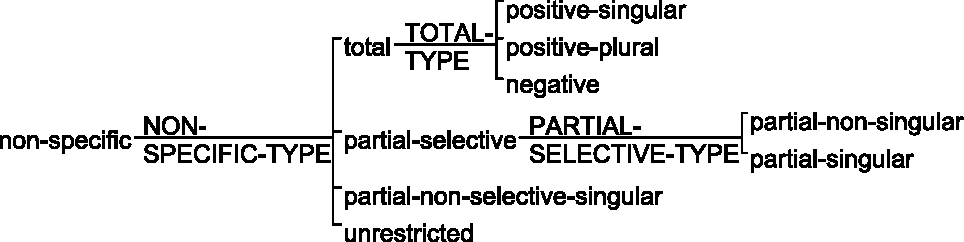
\includegraphics[width=0.9\linewidth]{Figures/SFL-grammar/determination-non-specific.pdf}
        \caption{The NON-SPECIFIC DETERMINATION system network}
        \label{fig:non-specific-deicticity}
    \end{figure}

    The dictionary lookup function outlined in Algorithm \ref{alg:dictionary-loockup} checks whether the word(s) of the CG node are in a dictionary. If the word is found then the function assigns the graph node with the associated features from the table. In addition, using the naive backwards induction method described in Algorithm \ref{alg:backward-induction-naive}, all the preselected features from a system network are determined and assigned to the graph node. %This works as a naive backwards induction of features from a delicate one up to the least delicate one at the root (see Algorithm \ref{alg:backward-induction-naive} in Section \ref{sec:system-networks-cs}). 
    An example of the dictionary is presented in the Table \ref{tab:lookup-dict-example} and the system network of NON-SPECIFIC determination is shown in Figure \ref{fig:non-specific-deicticity}.

\begin{table}[!ht]
    \centering
    \begin{tabular}{|l|l|}
        \hline
        \textit{Lexical item} & \textit{Feature}               \\ \hline
        a                     & partial-non-selective-singular \\ \hline
        all                   & positive-plural                \\ \hline
        either                & partial-singular               \\ \hline
        that                  & non-plural                     \\ \hline
    \end{tabular}
    \caption{Dictionary example for the NON-SPECIFIC DETERMINATION system network}
    \label{tab:lookup-dict-example}
\end{table}

    This section completed the explanation of how the MOOD features are assigned to the constituency graph. In the remainder of this chapter is addressed the task of assigning TRANSITIVITY process types and participant roles to the constituent units introduced in \citet{Costetchi2013}.

\section{Creation of empty elements}
\label{sec:creation-empty-elements}

    In the current work, when participants are missing but are syntactically recoverable in sentence then they are inferred from the structure and reference nodes are created for the missing elements. This phenomena is described in GB theory specifically as the \textit{Control and Binding} of empty elements \citep{Haegeman1991} introduced in Section \ref{sec:null-elements-gbt}. The \textit{reference constituents} are important for increasing the completeness and accuracy of semantic analysis by making the participants and their corresponding label explicit.

    This stage is particularly important for semantic role labelling because usually the missing elements are participant roles (theta roles) shaping the semantic configuration. The most frequent are the cases of \textit{control} where the understood subject of a clause is in the parent clause as in Examples \ref{ex:ctrl1}--\ref{ex:ctrl3} where \textit{Subj} is a generic subject placeholder introduced in Chapter \ref{ch:gbt} as \textit{PRO}, \textit{pro}, \textit{t-trace} and \textit{wh-trace}.

    \begin{exe}
    	\ex\label{ex:ctrl1}Poirot_i is considering whether [\textit{Subj_i} to abandon the investigation].
    	\ex\label{ex:ctrl2}Susan_i promised us [\textit{Subj_i} to help].
    	\ex\label{ex:ctrl3}They told you_i [\textit{Subj_i} to support the effort].
    \end{exe}

    There are also movement cases when a clause constituent receives no thematic role in a higher clause but one in a lower clause. The other case is of the non-overt constituents that are subjects in relative clauses and refer to the head of the nominal group. This part of the algorithm is set up to detect cases of \textit{null elements} as described in Section \ref{sec:placing-null-elements}, which relates GBT to Dependency Grammar and creates placeholder constituents for them which are in the next step enriched with semantic roles. Currently the NP traces and PRO subjects are created with a set of graph patterns, while the Wh traces are created with an algorithm.

\subsection{PRO and NP-trace Subjects}

    The \textit{xcomp} relation in DG can be encoded as a CG pattern graph (Figure \ref{fig:arb-control}) targeting the constituents that are non-finite clauses functioning as complement that have no subject constituent of their own and no ``if'' and ``for'' markers (according to generalisation \ref{gen:4}). They receive a PRO subject constituent (governed or not) by the parent clause subject.

    \begin{figure}[!ht]
    	\centering
    	\begin{tikzpicture}[tree-style,level distance=3em,level 1/.style={sibling distance=7em},] 
    	\node[pattern-node, anchor=center] (vb1){class:clause}
    	%child {node[pattern-node] (subj1) {class:nominal,\\element:subject,\\id:subj1}}
    	child {node[pattern-node,below = 2em of vb1,] (vb2) {element:complement,\\class:clause,\\finiteness:non-finite}
    		child {node[pattern-node-negative] (marker) {element:marker,\\words:[if,for]}}
    		child {node[pattern-node-negative] (subj2) {element:subject,\\operation:insert}}
    	};
    	\end{tikzpicture}
    	\caption{CG pattern for detecting PRO subjects}
    	\label{fig:arb-control}
    \end{figure}

    %%TODO either leave commented or rephrase
    %In terms SFG terms, if there is an Complement in the higher clause it is likely that it is the controller of the PRO in lower clause. Three role cognition verbs like in Example \ref{ex:pro7} take two complements where one of them is the phenomenon and can be a nominal group or a non-finite clause with PRO subject controlled by the object in higher clause.

    The generalisation \ref{gen:11} reflects criteria for selecting the controller of PRO based on its proximity in the higher clause. The schematic representation of the pattern for obligatory and subject object control (treated in Section \ref{sec:np-traces}) is depicted in Figures \ref{fig:obj-control} and \ref{fig:subj-control} respectively. In the case of Figure \ref{fig:subj-control} the prepositional complements do not affect subject control treatment in any way. The reason for that is because the graph pattern specifies only the nominal complements, which is complementary to object control pattern in Figure \ref{fig:obj-control}. %with respect to prepositional complements. 

    \begin{figure}[!ht]
    	\centering
    	\begin{tikzpicture}[tree-style,level distance=4em,level 1/.style={sibling distance=11em},] 
    	\node[pattern-node, anchor=center] (vb1){class:clause}
    	child {node[pattern-node] (subj1) {class:nominal,\\element:subject}}
    	child {node[pattern-node] (subj1) {class:nominal,\\element:complement,\\id:compl1}}
    	child {node[pattern-node] (vb2) {class:clause,\\element:complement,\\finiteness:non-finite}
    		child {node[pattern-node-negative] (marker) {element:marker,\\words:[if,for]}}
    		child {node[pattern-node-negative] (subj2) {element:subject,\\operation:insert,\\arg:\{id:compl1\}}}
    	};
    	\end{tikzpicture}
    	\caption{CG pattern for obligatory object control in complement clauses}
    	\label{fig:obj-control}
    \end{figure}
    
    \begin{figure}[!ht]
    	\centering
    	\begin{tikzpicture}[tree-style,level distance=4em,level 1/.style={sibling distance=11em},] 
    	\node[pattern-node, anchor=center] (vb1){class:clause}
    	child {node[pattern-node] (subj1) {class:nominal,\\element:subject,\\id:subj1}}
    	child {node[pattern-node-negative] (subj1) {class:nominal,\\element:complement}}
    	child {node[pattern-node] (vb2) {class:clause,\\element:complement,\\finiteness:non-finite}
    		child {node[pattern-node-negative] (marker) {element:marker,\\words:[if,for]}}
    		child {node[pattern-node-negative] (subj2) {element:subject,\\operation:insert,\\arg:\{id:subj1\}}}
    	};
    	\end{tikzpicture}
    	\caption{CG pattern for obligatory subject control in complement clauses}
    	\label{fig:subj-control}
    \end{figure}

    In dependency grammar the adjunct clauses are also introduced via \textit{xcomp} and \textit{prepc} relations, so syntactically there is no distinction between the two and patterns from Figures \ref{fig:obj-control} and \ref{fig:subj-control} are applicable.

    %%TODO introduce properly the discussion below about distinguishing the PRO and NP and about pre-marking the constituents with their potential to semantic roles

    %%todo this is discussed in sec:np-traces
    Before discussing each approach I would like to state that when the empty constituent is being created two important details are required: (a) the antecedent constituent it is bound to and (b) the type of relationship to its antecedent constituent or, if none is available, the type of empty element: t-trace or PRO. Now identifying the antecedent is quite easy and can be provided at the time of CG creation but since the empty element type may not always be available then it may have to be marked as partially defined.

    The first solution is to create the empty subject constituents based only on syntactic criteria, ignoring element type (either PRO or \textit{t}-trace) and hence postponing the decision to the semantic enrichment phase (addressed in this chapter). The advantage of doing this so is a clear separation of syntactic and semantic analysis. The empty subject constituents are created in the places where they should be and so this leaves aside the semantic concern of how the thematic roles are distributed. The disadvantage is leaving the created constituents incomplete or under-defined. Moreover the thematic role distribution must be done within the clause limits but because of raising, this process must be broadened to a larger scope beyond clause boundaries. This of course is an unwise approach as it might lead to unbounded dependencies and so unbounded complexity that needs to be addressed. 

    The second solution is to decide the element type before Transitivity analysis and remove the burden of complex patterns that go beyond clause borders. Also, all syntactic decisions would be made before semantic analysis and the empty constituents would be created fully defined with the binder and their type. But this means delegating semantically related decision to syntactic level (in a way peeking ahead in the process pipeline).

    In the current work, however, the semantic roles are addressed within the clause borders following the principle of one-main-verb-per-clause and thus avoiding the above mentioned risk of unbounded complexity. Also, the transitivity analysis is done based on pattern matching. This means a tremendous rise in complexity as the scope of a graph pattern is extended to two or more clauses. Instead, a desirable solution is iteration over all the clauses in the CG (a sentence) and matching semantic patterns within the clause boundaries one at a time.

    The solution adopted here is a mix of the two described above and addresses the issues of: (a) increasing the complexity of patterns for transitivity analysis, (b) leaving undecided which constituents accept thematic role in the clause and which do not. 

    The process to distinguish the empty constituent type starts by (a) identifying the antecedent and the empty element (through matching the subject control pattern in Figure \ref{fig:subj-control}), (b) identifying the main verbs of higher and lower clauses and correspondingly the set of possible configurations for each clause (by inquiry to the process type database (PTDB) described in the transitivity analysis Section \ref{sec:semantic-parsing}).

    If conditions from Generalisation \ref{gen:trace-detection} (from Section \ref{sec:np-traces}) are met then the empty constituent is a subject controlled \textit{t}-trace. Now we need a set of simple rules to mark which constituents receive a thematic role. These rules are  presented in Generalisation \ref{gen:thematic-marking} below.

    \begin{generalization}\label{gen:thematic-marking}
        Constituents receiving thematic roles are marked with a ``thematic-role'' label, those that do not receive a thematic role are marked with ``non-thematic-role'' and those that might receive thematic role with ``unknown-thematic-role''. So in each clause:
        \begin{itemize}
            \item the subject constituent is marked with thematic-role label unless (a) it is an expletive or (b) it is the antecedent of a \textit{t}-trace; then marked non-thematic-role
            \item a complement constituent that is an nominal group (NP) or an embedded complement clause is marked with thematic-role label.
            \item a  complement that is a prepositional group (PP) is marked with unknown-thematic-role.
            \item a complement that is a prepositional clause is marked with unknown-thematic-role label unless they are introduced via ``that'' and ``whether'' markers then it is marked with thematic-role label.
            \item the adjunct constituents are marked with non-thematic-role.
        \end{itemize}
    \end{generalization}

    According to Generalisation \ref{gen:9} PRO is optionally controlled in subject non-finite clauses. Since it is not possible to bind PRO solely on syntactic grounds Generalisation \ref{gen:9} proposed the arbitrary interpretation, i.e. no binding to an antecedent; and this is the solution adopted in this work for PRO elements.

    \begin{figure}[!ht]
    	\centering
    	\begin{tikzpicture}[tree-style,level distance=3em,level 1/.style={sibling distance=7em},] 
    	\node[pattern-node, anchor=center] (vb1){class:clause}
    	%	child {node[pattern-node] (subj1) {class:nominal,\\element:subject,\\id:subj1}}
    	%	child {node[pattern-node-negative] (subj1) {class:nominal,\\element:complement}}
    	child {node[pattern-node, below =2em of vb1, anchor=north] (vb2) {class:clause,\\element:subject,\\finiteness:non-finite}
    		child {node[pattern-node-negative, below =2em of vb2, anchor=north] (subj2) {element:subject,\\operation:insert,\\arg:\{words:one\}}}
    	};
    	\end{tikzpicture}
    	\caption{CG pattern for arbitrary control in subject clauses}
    	\label{fig:subj-arbitrary-control}
    \end{figure}

    The pattern for subject control in a subject clause  is represented in Figure \ref{fig:subj-arbitrary-control}. This of course is an oversimplification and more rigorous binding rules would need to be developed in future work to cover binding scenarios exemplified in Examples \ref{ex:pro12}--\ref{ex:pro15}.

\subsection{Wh-trances}
    Creating constituents for Wh-traces involved a slightly larger number of scenarios and for pragmatic reasons I implemented the following algorithm rather than create the set of corresponding graph patterns. Nevertheless in future work this should be expressed as graph patterns in order to be consistent with the general approach of the thesis. Algorithm \ref{alg:create-wh-trace} shows how it is currently done.

    \begin{algorithm}[!ht]
    	\Input { \cg}
    	\Begin{
            \If {more than one clause in \cg}
            {
           		\For {\Element \KwTo list of Wh-elements in \cg}
           			{
           				identify the Wh-groups containing the \Element\;
           				identify the syntactic function of the Wh-element within the group\;
           				identify the function of Wh-group in the clause\;
           				%check the number of clauses and which of clauses contains the Wh-group\;
        				\For(low to high){\Group \KwTo \cg}
        					{\If{Wh-group is \textbf{not} Subject \textbf{AND}\\ Wh-group is \textbf{not} in lowest embedded clause}
        						{
        						\eIf{Wh-group is Adjunct function}
        						{create Adjunct Wh-trace using \dg and \cg}
        						{create Theta Wh-trance using \dg and \cg}
        						}
        					}	
           			}
    		}
    	}
    	\caption{Creating the Wh-traces}
    	\label{alg:create-wh-trace}
    \end{algorithm}

    The first line of the algorithm checks if there are more than one clause in the CG, otherwise it cannot continue. Then all the Wh-elements, their functions within the group and the clause identified. Then, from the lower to higher, clauses are iterated and the constituent corresponding to Wh-trace in the lower clause is created and linked to the trace constituent in the parent clause. The creation of the Adjunct or Theta Wh-traces involves different procedures. The corresponding algorithms have been omitted in this section but are included in the Appendix \ref{ch:extra-pseudo-code}. 

    After the null elements are created the constituency graph is ready for the semantic enrichment stage, and semantic configurations are assigned to each clause. The next sections introduce first how the PTDB has been normalised and how the graph patterns are created from it; they then proceed with the semantic enrichment algorithm.

\section{Cleaning up the PTDB}
\label{sec:claning-ptdb}

    The original version of the PTDB available on Neale's personal page\footnote{see \url{http://www.itri.brighton.ac.uk/~Amy.Neale/}} is not usable for computational purposes as such. It  contains records applying a couple of different notations and sometimes informal comments for human understanding, which from a machine standpoint are noise and cannot be processed as such. In this section I explain how the original PTDB was transformed into a machine readable form in order to be used as a lexical database.

    The internal structure of the PTDB is detailed in Neale's PhD thesis \citep[193--231]{Neale2002}. Here I focus on three columns which are of interest for the parsing process: the \textit{verb form} ($1^{st}$), the Cardiff grammar \textit{process type} ($6^{th}$) and the participant role \textit{configuration} ($8^{th}$). Note that column numbers correspond to the original PTDB structure. After the transformation the PTDB column descriptions are as described in Table \ref{tab:ptdb-comparison}. The field names in italics are the ones of interest and have been modified.

    \begin{table}[!ht]
    	\centering
    	\begin{tabulary}{\textwidth}{|l|L|L|}
    		\hline
    		\textbf{Column} & \textbf{Original}                    & \textbf{Modified}                                         \\ \hline
    		1/A             & Form                                 & Form                                                      \\ \hline
    		2/B    & \textit{Occurences of form}          & \textit{Occurences of form}                               \\ \hline
    		3/C             & COB class (\& figure where possible) & COB class (\& figure where possible)                      \\ \hline
    		4/D             & meaning descrition                   & meaning descrition                                        \\ \hline
    		5/E             & Occurences in 5 million words        & Occurences in 5 million words                             \\ \hline
    		6/F    & \textit{Cardiff Grammar feature}     & \textit{Cardiff Grammar process type (reindexed/renamed)} \\ \hline
    		7/G             & Levin Feature                        & \textit{Cardiff participant feature}                      \\ \hline
    		8/H             & \textit{Participant Role Configuration}       & \textit{Cardiff participant feature (extra)}              \\ \hline
    		9/I             & Notes                                & Levin feature                                             \\ \hline
    		10/J            &                                      & \textit{Participant Role Configuration}                   \\ \hline
    		11/K            &                                      & Notes                                                     \\ \hline
    	\end{tabulary}
    	\caption{The table structure of PTDB before and after the transformation}
    	\label{tab:ptdb-comparison}
    \end{table}

    Next I describe the transformed PTDB and how it is interpreted. For a start, the verb form column contains either the base form of the verb (e.g. draw, take), base form plus a preposition (e.g. draw into, draw away, take apart, take away from) or the base form plus a phraseologic expression (e.g draw to an end, take on board, take the view that, take a shower). The prepositions are either the verbal particles or the preposition introducing the prepositional phrase complement. Prepositions often influence the process type and the participant configuration. So they are important cues to consider during semantic role assignment. The verb forms that have the same process type and configuration but different prepositions are often grouped together delimited by a slash ``/'' (e.g. draw into/around, take off/on) or if optional (i.e. coincide with the meaning of the verb base form without any preposition), they are placed in round brackets ``()'' (e.g. flow (into/out/down) ).

    The process type column registers one feature from the PROCESS-TYPE systemic network depicted in Figure \ref{fig:cardiff-transitivity}, which was introduced in Section \ref{sec:transitivity}. The participant configuration column contains a sequence of participant type abbreviations joined by a plus sign ``+'' (e.g. Ag + Af, Em + Ph, Ag-Cog + Ph). The order of participants corresponds to the Active voice in Declarative mood, also called the \textit{canonical form of a configuration} described in \citet{Fawcett2009}. Originally the configurations contained the ``Pro'' abbreviation signifying the place of the main verb/process. As all configurations are in canonical form, the Pro was redundant occurring always in the second position thus has been removed. So the first participant, in canonical form, corresponds to the Subject, the second to the first complement and the third to the second complement. Some participants are optional for the meaning and are marked with round brackets ``()'', e.g. Ag + Af-Ca (+ Des), meaning that the participant may or may not be realised. Sometimes, for directional or locational process types, the second or third participants may function as Adjuncts, which currently complicates the matching process.

    Not all the records in the original resource fulfil the description above and so needed corrections. For example when Neale had doubts during the making of PTDB, she marked uncertainties with a question mark ``?''. In addition, the ``,'' (comma) and ``\&'' (and) signs are used inconsistently with various meaning in all columns. Also, comments such as ``not in Cob'' (i.e. not in Cobuild presumably) were encountered in several columns.

    Some records contain only prepositions listed in the verb form column, which actually represents omissions of the main verb that is to be found in the immediately preceding records(s); this have been fixed by pre-pending the verb form to the preposition. 

    %The account of verb meanings in PTDB is not exhaustive. Compared to VerbNet or FrameNet there are considerably less meanings described. 

    Among the identified verb meanings in PTDB, there are also some that do not contain configurations. These records missing a process type and configuration have been suppressed. 

    The process type feature column contained originally a second feature which has been removed; it represented a compressed version of the participant configuration and it was redundant as the full configuration is registered in the next column. 

    In the PTDB Neale uses the slightly different process type names than the ones used in this work. The process type features have been thus re-indexed and adapted to match exactly the feature labels in the PROCESS-TYPE systemic network (e.g. ``one role action'' became ``one-role-action'', ``emotion plus xxx'' became ``emotive'', ``cognition xxx'' became ``two-role-cognition''). Appendix \ref{ch:reindexing-ptdb} provides the mapping across the process type versions. 

    The configuration column is one of the most important in the PTDB. Checking its consistency with respect to Fawcett's Transitivity system revealed the need for some corrections. For example ``Af + Af'', ``Af-Ca + Pos + Ag'', ``Af-Cog + Ph + Ag'' are grammatically impossible configurations and were manually corrected to the closest likely configuration ``Ag + Af'', ``Ag + Af-Ca + Pos'', ``Ag + Af-Cog + Ph''.

    Other records, judged by the process type, were incomplete. For example instances of two role actions registered only one of the roles, e.g. Af or Ca omitting the Ag participant. These records have also been manually corrected by prepending the Ag, Ag-Af or Cog roles depending as appropriate. 

    %\begin{figure}[!ht]
    %    \centering
    %    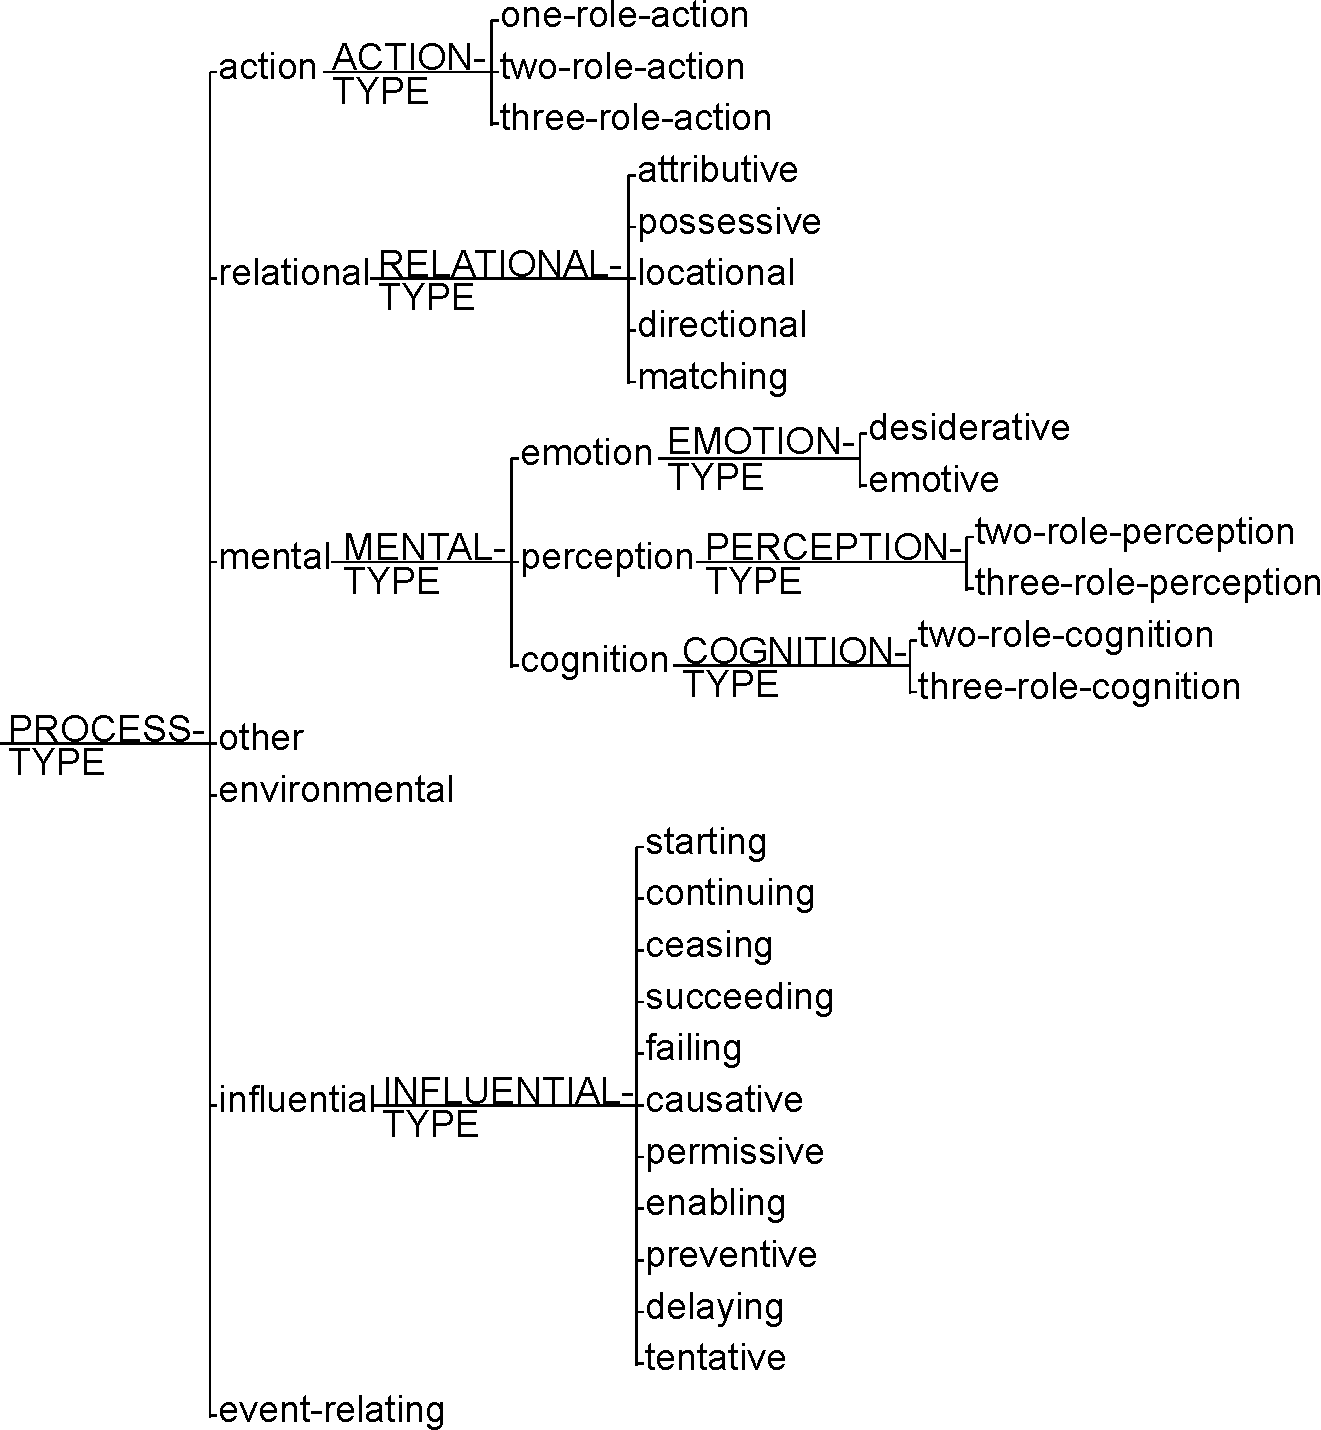
\includegraphics[width=0.7\linewidth]{Figures/SFL-grammar/Transitivity}
    %    \caption{TRANSITIVITY system network in Cardiff Grammar} %[TRANSITIVITY system network in Cardiff Grammar]
    %    \label{fig:transitivity-system}
    %\end{figure}

    The ``Dir'' participant is interpreted as direction but is not registered/defined in the Cardiff Grammar. Nevertheless there is a ``Des'' participant which I believe is the closest match. Therefore all ``Dir'' occurrences have been changed to ``Des''. One may argue that the two have different meanings however grammatically they seem to behave the same (at least in the accounted configurations). 

    By contrast some process types have been changed from action into either locational or directional because they contained either ``Loc'' (location), ``Des'' (destination) or ``So'' (source) participants which are not found in action processes unless they function as adjuncts, which are out of the context of the current description.

    A note worth making here is that locational, movement specifically but also other spatial verbs are very difficult to assign roles correctly because their participants are locations, directions, destinations etc., which can also serve as spatial adjuncts. This aspect has not been directly addressed in present work and is reflected in the evaluation results (that will be presented in Chapter \ref{ch:evaluation}) with a lower accuracy for these process types than others.

    The Cardiff features column indicates the process type selected in the TRANSITIVITY system corresponding to one of the top levels depicted in Figure \ref{fig:cardiff-transitivity} provided in Chapter \ref{ch:the-grammar}. Next section provides a description of how the graph patterns are generated from the PTDB. 

\section{Generation of the TRANSITIVITY graph patterns}
\label{sec:gen-sem}
    The configuration pattern graphs are used for CG enrichment executed through graph matching operation as described in Section \ref{sec:graph-matching}. In the previous section we saw how the PTDB has been cleaned up and normalised to support automatic generation of the \textit{Configuration Graph Patterns} (CGP), which afterwards are used to enrich constituency graphs with transitivity features. These graph patterns represent a constrained syntactic structure that carries semantic features that  are applied if the pattern is identified. 

    CGPs are generated from the process type and participant configuration columns of the PTDB. Figure \ref{fig:general-configuration-canonic} depicts the prototypical template for generating a three role CGP for canonical participant order that is active VOICE and declarative MOOD. This pattern matches declarative clause with a subject and two complements and in case of success updates the constituents with process type and participant roles. When the configuration has only one or two participants the graph pattern indicates one or two negative complement nodes as depicted in Figures \ref{fig:general-configuration-canonic-two} and \ref{fig:general-configuration-canonic-one-partic}. In this section I do not aim at providing an exhaustive account of all the pattern forms but explain the principles by which they are automatically generated.

    \begin{figure}[!ht]
    	\centering
    	\begin{tikzpicture}[tree-style, level distance=4em, level 1/.style={sibling distance=12em},] 
    	\node[pattern-node, anchor=center] (proc){class:clause,\\MOOD:declarative, VOICE:active\\operation:update,\\ arg1:\{process:process-type\}}
    	child{node[pattern-node]{element:subject,\\operation:update,\\ arg1:\{participant:role1\}} edge from parent node[left] {}}
    	child{node[pattern-node]{element:complement,\\operation:update,\\ arg1:\{participant:role2\}} edge from parent node[below] {}}
    	child{node[pattern-node]{element:complement,\\operation:update,\\ arg1:\{participant:role3\}} edge from parent node[right] {}};
    	\end{tikzpicture}
    	\caption{Declarative MOOD and active VOICE graph pattern with three participant roles}
    	\label{fig:general-configuration-canonic}
    \end{figure}
    
    \begin{figure}[!ht]
    	\centering
    	\begin{tikzpicture}[tree-style, level distance=4em, level 1/.style={sibling distance=12em},] 
    	\node[pattern-node, anchor=center] (proc){class:clause,\\MOOD:declarative, VOICE:active\\operation:update,\\ arg1:\{process:process-type\}}
    	child{node[pattern-node]{element:subject,\\operation:update,\\ arg1:\{participant:role1\}} edge from parent node[left] {}}
    	child{node[pattern-node]{element:complement,\\operation:update,\\ arg1:\{participant:role2\}} edge from parent node[below] {}}
    	child{node[pattern-node-negative]{element:complement} edge from parent node[below] {}};
    	\end{tikzpicture}
    	\caption{Declarative MOOD and active VOICE graph pattern with two participant roles}
    	\label{fig:general-configuration-canonic-two}
    \end{figure}
    
    \begin{figure}[!ht]
        \centering
        \begin{tikzpicture}[tree-style, level distance=4em, level 1/.style={sibling distance=12em},] 
        \node[pattern-node, anchor=center] (proc){class:clause,\\MOOD:declarative, VOICE:active\\operation:update,\\ arg1:\{process:process-type\}}
        child{node[pattern-node]{element:subject,\\operation:update,\\ arg1:\{participant:role1\}} edge from parent node[left] {}}
        child{node[pattern-node-negative]{element:complement} edge from parent node[below] {}}
        child{node[pattern-node-negative]{element:complement} edge from parent node[right] {}};
        \end{tikzpicture}
        \caption{Declarative MOOD and active VOICE graph pattern with one participant role}
        \label{fig:general-configuration-canonic-one-partic}
    \end{figure}

    Besides the canonical CGP a set of variations are generated for each configuration corresponding to yes-no and Wh-Subj/Wh-obj/Wh-adj interrogative forms, imperative form and to passive voice form. 
    %The variations are function of the process type, participant roles, mood and voice. 
    When each of the variants are supported by the process type and participant configuration, the following CGP are generated: (1) the declarative active (2) the passive (3) the imperative and (4) Wh-interrogative (Wh-Subj/Wh-obj/Wh-adj especially important for locational and directions processes).

    %\explain{how do the process type influence the generated forms and also how the participant roles influence the forms?}
    %\explain{How do the CGP vary according to other features such as voice and mood}
    %\explain{What happens in Wh-Subj/Wh-obj/Wh-adj? what happens in Wh-YN, how are the patterns generated to cove those?}
    
    If the configuration accepts passive voice, i.e. the first participant in the configuration is not the expletive ``there'' or the pleonastic ``it'' and the last role is not Agent role, then both active and passive voice CPG are generated. Otherwise the passive form is not possible. 

    The imperative form CGP is generated if the first role of the configuration implies an active animate entity. Thus the nominal features of the subject must already be provided. Roles that accept imperative form are: Agent, Emoter, Cognizant, Perceiver and their compositional derivations, e.g. Agent-Carrier, Agent-Cognizant, Affected-Emoter etc. Clausal subjects are excluded. 

    The passive differs from the active voice pattern by switching the places of the first two roles resulting in the second role matched to the subject function and the first role to the first complement. In the case of imperative, the first role  as well as the subject constituent are simply omitted.  

    Algorithm \ref{alg:generating-cpg} outlines how the CPGs are generated from the PTDB. The CPGs are represented as Python structures and are stored in a Python module. This way the graph patterns are accessible as native structures making it easy to instantiate and execute the graph patterns. The process types are also grouped by the process type and number of participants which reduces the number of patterns be match per clause.  

    \begin{algorithm}[!ht]
    	\Input { PTDB }
    	\Begin{
    		generate unique set of process type + participant roles\;
    		generate unique set of process types\;
    		\For{process type \KwTo possible process type}
    		{
    			%generate configuration set for given process type \;
    			\For{configuration \KwTo configuration set}
    			{
    				generate declarative active pattern graph \;
    				\If {no expletive in configuration}
    				{
    					\If{configuration accepts passive}
    					{
    						generate declarative passive pattern graph\;
    					}
    					\If{configuration accepts imperative}
    					{
    						generate imperative pattern graph\;
    					}
    					\If{locational process}
    					{
    					generate expletive there pattern graph \;
    					}
    					\If{configuration participants may function as Adjuncts}
    					{
    						\tcc{the Directional processes varying optional Source, Path and Destination}
    						generate variate role indicative active pattern graphs \;
    						generate variate role indicative passive pattern graphs \;
    						generate variate role imperative pattern graphs \;
    						generate variate role Wh-interrogative pattern graphs \;
    					}
    				}
    			}
    		}
    	}
    	\caption{Generating the CPGs from the PTDB}
    	\label{alg:generating-cpg}
    \end{algorithm}

    The first two lines of the algorithm synthesise the PTDB by grouping unique configurations for each process type. Then for each configuration of each process type one to three pattern graphs depending on the configuration and process type specifics are generated.

    \begin{figure}[!ht]
    	\centering
    	\begin{tikzpicture}[tree-style, level distance=4em, level 1/.style={sibling distance=12em},] 
    	\node[pattern-node, anchor=center] (proc){class:clause,\\MOOD:declarative, VOICE:passive\\operation:update,\\ arg1:\{process:process-type\}}
    	child{node[pattern-node]{element:subject,\\operation:update,\\ arg1:\{participant:Role2\}} edge from parent node[left] {}}
    	child{node[pattern-node]{element:complement,\\operation:update,\\ arg1:\{participant:Role1\}} edge from parent node[below] {}}
    	child{node[pattern-node]{element:complement,\\operation:update,\\ arg1:\{participant:Role3\}} edge from parent node[right] {}};
    	\end{tikzpicture}
    	\caption{Declarative MOOD and passive VOICE graph pattern with three participant roles}
    	\label{fig:general-configuration-passive}
    \end{figure}
    
    \begin{figure}[!ht]
    	\centering
    	\begin{tikzpicture}[tree-style, level distance=4em, level 1/.style={sibling distance=12em},]
    	\node[pattern-node, anchor=center] (proc){class:clause,\\MOOD:imperative, operation:update,\\ arg1:\{process:process-type\}}
    	child{node[pattern-node-negative]{element:subject} edge from parent node[left] {}}
    	child{node[pattern-node]{element:complement,\\operation:update,\\ arg1:\{participant:Role2\}} edge from parent node[below] {}}
    	child{node[pattern-node]{element:complement,\\operation:update,\\ arg1:\{participant:Role3\}} edge from parent node[right] {}};
    	\end{tikzpicture}
    	\caption{Imperative MOOD graph pattern with three participant roles}
    	\label{fig:general-configuration-imperative}
    \end{figure}

    %\todo{Explain the rules by which are created variations on voice, mood (and other features) based on configuration type and participants}
    The declarative MOOD active VOICE pattern (depicted in Figure \ref{fig:general-configuration-canonic}) corresponding to the canonical form in PTDB is always generated. If the configuration does not contain an expletive and accepts passive voice then the corresponding pattern is generated with the first and second roles switched as in Figure \ref{fig:general-configuration-passive}. Note that role2 is assigned to the subject and role1 to the first complement. If the configuration accepts imperatives, then also a subject-less pattern graph is generated with the first role omitted as depicted in Figure \ref{fig:general-configuration-imperative}. 

    Directional processes are a special case. Examples \ref{ex:directional2} to \ref{ex:directional4} are equally valid configurations. Example \ref{ex:directional5} is a generic representation highlighting the optionality of these participants. 
    %\todo{Discuss Neale/Fawcett possible configurations}
    \begin{exe}
    	\ex\label{ex:directional2} The parcel travelled from London[So].
    	\ex\label{ex:directional3} The parcel travelled via Poland[Pa].
    	\ex\label{ex:directional4} The parcel travelled to Moscow[Des].
    	\ex\label{ex:directional5} The parcel travelled (from London[So]) (via Poland[Pa]) (to Moscow[Des]).
    \end{exe}

    And so in directional configurations, second, third and fourth participants are optional and may occur in any order, but at least one of them should be present. Therefore So, Pa and Des participants patterns should be generated for all combinations as presented in Table \ref{tab:directional-partic-variations}.

    \begin{table}[!ht]
    	\centering
    	\begin{tabular}{|c|c|c|}
    		\hline
    		\textbf{So} & \textbf{Pa} & \textbf{Des} \\ \hline
    		\textbf{+} & - & - \\ \hline
    		- & \textbf{+} & - \\ \hline
    		- & - & \textbf{+} \\ \hline
    		\textbf{+} & \textbf{+} & - \\ \hline
    		\textbf{+} & - & \textbf{+} \\ \hline
    		- & \textbf{+} & \textbf{+} \\ \hline
    		\textbf{+} & \textbf{+} & \textbf{+} \\ \hline
    	\end{tabular}
    	\caption{Participant arrangements for Directional processes (order independent)}
    	\label{tab:directional-partic-variations}
    \end{table}

    Finally, the CPGs are grouped by process type. This alleviates the burden of selecting the number of patterns to test for a certain clause. 

    %The python structure looks as represented in Listing \ref{lst:config-pattern-set}
    %\begin{lstlisting}[language=json,firstnumber=1, caption={Configuration Pattern Set as a Python dictionary structure},label={lst:config-pattern-set}]
    %configuration_pattern_set = {
    %	process_type1 : {
    %		config1 : [pattern1, panttern2,...],
    %		config2 : [pattern3, panttern4,...],
    %	},
    %	process_type2 : {
    %		config3 : [pattern5, panttern6,...],
    %		config4 : [pattern7, panttern8,...],
    %	}
    %	...
    %}
    %\end{lstlisting}

    The patterns are generated in advance and so at runtime are ready for execution. This decreases execution time. Next follows the description of how the generated configuration graph patterns are used in the Transitivity enrichment phase.

\section{Enrichment with TRANSITIVITY features}
\label{sec:semantic-parsing}

    Once the constituency graph has been enriched with MOOD and nominal DEIXIS features and the null elements created, it is ready to be enriched with TRANSITIVITY features. The algorithm identifies, in each clause, the main verb and the potential participant constituents and searches in the PTDB for the lexical item matching the main verb and any of its extensions filtering (based on the clause constituency) the possible configurations for the verb (comprising all the verb configurations). Then all the graph patterns corresponding to the possible configurations are executed on the clause, which, if matched, will enrich the clause CG. 

    \begin{algorithm}[!ht]
        \Input { \cg, \dg }
        \Begin
        {
            \For{ clause \KwTo clauses in mcg}
            {
                select from PTDB candidate process types and configurations\;
                filter configurations fitting the clause \;
                \For{config \KwTo valid possible configurations}
                {
                    filter pre-generated pattern graphs of the config fitting the clause\;
                    \For{pattern \KwTo filtered pattern graph set}
                    {
                        \label{line:enrich-from-pattern} enrich clause using pattern and mcg filtered by role constraints\;
                    }
                }
            }
        }
        \caption{Transitivity parsing}
        \label{alg:transitivity-parsing}
    \end{algorithm}

    Algorithm \ref{alg:transitivity-parsing} outlines the semantic parsing process implemented in the current parser which is a cascade of three loops. The first loop iterates through clauses in the mood constituency graph and for each the candidate process types are identified by considering: (a) the main verb, (b) the prepositions connected to it (either prepositional particles, or prepositions introducing a complement or adjunct prepositional phrase listed in Table \ref{tab:participant-roles-constraints}) or (c) phrasal expressions such as ``take a shower'' which were explained in Section \ref{sec:ptdb-description-technical}.

    \begin{table}[!ht]
    	\centering
    	\begin{tabular}{|l|l|}
    		\hline
    		\textbf{Role} & \textbf{Prepositions}             \\ \hline
    		Des           & to,towards,at,on,in,              \\ \hline
    		Ben           & to,for,                           \\ \hline
    		Attr          & as,                               \\ \hline
    		Ra            & on,in,                            \\ \hline
    		So            & from,                             \\ \hline
    		Pa            & through,via,                      \\ \hline
    		Loc           & in,at,into,behind,in front of, on \\ \hline
    		Mtch          & with,to,                          \\ \hline
    		Ag            & by,                               \\ \hline
    		Ph            & about,                            \\ \hline
    		Cog           & to                                \\ \hline
    	\end{tabular}
    	\caption{Prepositional constraints on participant roles }
    	\label{tab:participant-roles-constraints}
    \end{table}

    The second loop iterates through the candidate configurations for each candidate process type and selects the graph patterns that should be matched to the current clause. Then iteratively, each of the retrieved graph patterns (in the third loop) are applied to the clause graph. Line \ref{line:enrich-from-pattern} enriches CG nodes with new features of the pattern graph each time they are successfully matched. Before enrichment the CG nodes are checked against an additional set of conditions (captured by Algorithm \ref{alg:role-constraint-check}) which were omitted in the pattern graph. These conditions may prevent enrichment even if the pattern has been identified. 

    %\explain{What is the selection/filtering based on ? probably subj/role, preposition/role constraints} The last set of checks is an attempt to reduce the false positive assignments. 
    %%For example if the complement is a clause then it can take only Phenomena role otherwise the entire

    \begin{algorithm}[!ht]
    	\Input {\node, role, \dg }
    	\Begin
    	{
    		\tcc{Cog, Em and Perc must be animates}
    		\If{role is Cog \textbf{or} Em \textbf{or} Perc}
    		{
    			check that the \node has animate feature \;
    		}
    		\tcc{clauses can only be phenomenas}
    		\If{\node is a clause}{
    			check that role is Ph only \;
    		}
    		\tcc{prepositional phrases can only start with certain prepositions for a role}
    		\If{\node is a Prepositional Phrase}
    		{
    			get the list of allowed prepositions for the role \;
    			check if the prepositional phrase starts with any of the allowed prepositions \;
    		}
    	}
    	\caption{Participant Role constraint check if a role is not illegal for constituent}
    	\label{alg:role-constraint-check}
    \end{algorithm}

    % The Transitivity parsing results in multiple process configurations being assigned to clauses decreasing, in a way, precision and or introducing uncertainty. Because the final result contains few possibilities without knowing which one is the case. This uncertainty, decreased with several heuristics, is not dealt with by the current parser and shall be addressed in the future work. 

\section{Summary}
%todo larger section

    This chapter has described how the constituency backbone is enriched with syntactic and semantic features from the MOOD and TRANSITIVITY system networks using graph patterns. Besides the core sections describing the enrichment algorithms, this chapter provides explanations about the graph pattern creation, CG extension with null elements and the clean-up of PTDB

    First null elements are identified and filled with proxy constituents. This process ensures higher accuracy of semantic role assignments from the configuration patterns in the second step. 

    The configuration patterns have been generated from the PTDB - a verb database accounting for Transitivity patterns in Cardiff grammar. In order to generate these patterns the PTDB had first to be cleaned up, unified and aligned to the present Transitivity system. Then for each configuration a set of possible patterns were generated, which vary based on mood, voice, process type and participants. Finally the semantic role labelling step employs the same pattern based enrichment mechanism as used in Section \ref{sec:enrichment-stage}.

    The algorithms can be improved by externalisation of constraints and conditions. In the next iterations of Parsimonious Vole parser development should be towards higher abstraction and separation between the grammatical constraints (in SFL represented as systemic realisation rules) and the algorithm.
